% Options for packages loaded elsewhere
\PassOptionsToPackage{unicode}{hyperref}
\PassOptionsToPackage{hyphens}{url}
%
\documentclass[
  ignorenonframetext,
]{beamer}
\usepackage{pgfpages}
\setbeamertemplate{caption}[numbered]
\setbeamertemplate{caption label separator}{: }
\setbeamercolor{caption name}{fg=normal text.fg}
\beamertemplatenavigationsymbolsempty
% Prevent slide breaks in the middle of a paragraph
\widowpenalties 1 10000
\raggedbottom
\setbeamertemplate{part page}{
  \centering
  \begin{beamercolorbox}[sep=16pt,center]{part title}
    \usebeamerfont{part title}\insertpart\par
  \end{beamercolorbox}
}
\setbeamertemplate{section page}{
  \centering
  \begin{beamercolorbox}[sep=12pt,center]{part title}
    \usebeamerfont{section title}\insertsection\par
  \end{beamercolorbox}
}
\setbeamertemplate{subsection page}{
  \centering
  \begin{beamercolorbox}[sep=8pt,center]{part title}
    \usebeamerfont{subsection title}\insertsubsection\par
  \end{beamercolorbox}
}
\AtBeginPart{
  \frame{\partpage}
}
\AtBeginSection{
  \ifbibliography
  \else
    \frame{\sectionpage}
  \fi
}
\AtBeginSubsection{
  \frame{\subsectionpage}
}
\usepackage{lmodern}
\usepackage{amssymb,amsmath}
\usepackage{ifxetex,ifluatex}
\ifnum 0\ifxetex 1\fi\ifluatex 1\fi=0 % if pdftex
  \usepackage[T1]{fontenc}
  \usepackage[utf8]{inputenc}
  \usepackage{textcomp} % provide euro and other symbols
\else % if luatex or xetex
  \usepackage{unicode-math}
  \defaultfontfeatures{Scale=MatchLowercase}
  \defaultfontfeatures[\rmfamily]{Ligatures=TeX,Scale=1}
\fi
% Use upquote if available, for straight quotes in verbatim environments
\IfFileExists{upquote.sty}{\usepackage{upquote}}{}
\IfFileExists{microtype.sty}{% use microtype if available
  \usepackage[]{microtype}
  \UseMicrotypeSet[protrusion]{basicmath} % disable protrusion for tt fonts
}{}
\makeatletter
\@ifundefined{KOMAClassName}{% if non-KOMA class
  \IfFileExists{parskip.sty}{%
    \usepackage{parskip}
  }{% else
    \setlength{\parindent}{0pt}
    \setlength{\parskip}{6pt plus 2pt minus 1pt}}
}{% if KOMA class
  \KOMAoptions{parskip=half}}
\makeatother
\usepackage{xcolor}
\IfFileExists{xurl.sty}{\usepackage{xurl}}{} % add URL line breaks if available
\IfFileExists{bookmark.sty}{\usepackage{bookmark}}{\usepackage{hyperref}}
\hypersetup{
  pdftitle={Hydrological Modelling and R},
  pdfauthor={Emanuele Cordano},
  hidelinks,
  pdfcreator={LaTeX via pandoc}}
\urlstyle{same} % disable monospaced font for URLs
\newif\ifbibliography
\usepackage{color}
\usepackage{fancyvrb}
\newcommand{\VerbBar}{|}
\newcommand{\VERB}{\Verb[commandchars=\\\{\}]}
\DefineVerbatimEnvironment{Highlighting}{Verbatim}{commandchars=\\\{\}}
% Add ',fontsize=\small' for more characters per line
\usepackage{framed}
\definecolor{shadecolor}{RGB}{248,248,248}
\newenvironment{Shaded}{\begin{snugshade}}{\end{snugshade}}
\newcommand{\AlertTok}[1]{\textcolor[rgb]{0.94,0.16,0.16}{#1}}
\newcommand{\AnnotationTok}[1]{\textcolor[rgb]{0.56,0.35,0.01}{\textbf{\textit{#1}}}}
\newcommand{\AttributeTok}[1]{\textcolor[rgb]{0.77,0.63,0.00}{#1}}
\newcommand{\BaseNTok}[1]{\textcolor[rgb]{0.00,0.00,0.81}{#1}}
\newcommand{\BuiltInTok}[1]{#1}
\newcommand{\CharTok}[1]{\textcolor[rgb]{0.31,0.60,0.02}{#1}}
\newcommand{\CommentTok}[1]{\textcolor[rgb]{0.56,0.35,0.01}{\textit{#1}}}
\newcommand{\CommentVarTok}[1]{\textcolor[rgb]{0.56,0.35,0.01}{\textbf{\textit{#1}}}}
\newcommand{\ConstantTok}[1]{\textcolor[rgb]{0.00,0.00,0.00}{#1}}
\newcommand{\ControlFlowTok}[1]{\textcolor[rgb]{0.13,0.29,0.53}{\textbf{#1}}}
\newcommand{\DataTypeTok}[1]{\textcolor[rgb]{0.13,0.29,0.53}{#1}}
\newcommand{\DecValTok}[1]{\textcolor[rgb]{0.00,0.00,0.81}{#1}}
\newcommand{\DocumentationTok}[1]{\textcolor[rgb]{0.56,0.35,0.01}{\textbf{\textit{#1}}}}
\newcommand{\ErrorTok}[1]{\textcolor[rgb]{0.64,0.00,0.00}{\textbf{#1}}}
\newcommand{\ExtensionTok}[1]{#1}
\newcommand{\FloatTok}[1]{\textcolor[rgb]{0.00,0.00,0.81}{#1}}
\newcommand{\FunctionTok}[1]{\textcolor[rgb]{0.00,0.00,0.00}{#1}}
\newcommand{\ImportTok}[1]{#1}
\newcommand{\InformationTok}[1]{\textcolor[rgb]{0.56,0.35,0.01}{\textbf{\textit{#1}}}}
\newcommand{\KeywordTok}[1]{\textcolor[rgb]{0.13,0.29,0.53}{\textbf{#1}}}
\newcommand{\NormalTok}[1]{#1}
\newcommand{\OperatorTok}[1]{\textcolor[rgb]{0.81,0.36,0.00}{\textbf{#1}}}
\newcommand{\OtherTok}[1]{\textcolor[rgb]{0.56,0.35,0.01}{#1}}
\newcommand{\PreprocessorTok}[1]{\textcolor[rgb]{0.56,0.35,0.01}{\textit{#1}}}
\newcommand{\RegionMarkerTok}[1]{#1}
\newcommand{\SpecialCharTok}[1]{\textcolor[rgb]{0.00,0.00,0.00}{#1}}
\newcommand{\SpecialStringTok}[1]{\textcolor[rgb]{0.31,0.60,0.02}{#1}}
\newcommand{\StringTok}[1]{\textcolor[rgb]{0.31,0.60,0.02}{#1}}
\newcommand{\VariableTok}[1]{\textcolor[rgb]{0.00,0.00,0.00}{#1}}
\newcommand{\VerbatimStringTok}[1]{\textcolor[rgb]{0.31,0.60,0.02}{#1}}
\newcommand{\WarningTok}[1]{\textcolor[rgb]{0.56,0.35,0.01}{\textbf{\textit{#1}}}}
\usepackage{longtable,booktabs}
\usepackage{caption}
% Make caption package work with longtable
\makeatletter
\def\fnum@table{\tablename~\thetable}
\makeatother
\usepackage{graphicx}
\makeatletter
\def\maxwidth{\ifdim\Gin@nat@width>\linewidth\linewidth\else\Gin@nat@width\fi}
\def\maxheight{\ifdim\Gin@nat@height>\textheight\textheight\else\Gin@nat@height\fi}
\makeatother
% Scale images if necessary, so that they will not overflow the page
% margins by default, and it is still possible to overwrite the defaults
% using explicit options in \includegraphics[width, height, ...]{}
\setkeys{Gin}{width=\maxwidth,height=\maxheight,keepaspectratio}
% Set default figure placement to htbp
\makeatletter
\def\fps@figure{htbp}
\makeatother
\setlength{\emergencystretch}{3em} % prevent overfull lines
\providecommand{\tightlist}{%
  \setlength{\itemsep}{0pt}\setlength{\parskip}{0pt}}
\setcounter{secnumdepth}{-\maxdimen} % remove section numbering
%% EMOS rmarkdown/beamer header
%% Mark van der Loo (2016)
\usepackage{listings}
\usepackage{mdframed}
\usepackage{tikz}

\usetikzlibrary{arrows, positioning, decorations.pathreplacing} 
\usepackage{pgfplots}
\usepackage{color}


% CBS corporate light blue
\definecolor{corplightblue}{HTML}{00a1cd}
% CBS corporate dark blue
\definecolor{corpdarkblue}{HTML}{0058b8}

% set title colors
\setbeamercolor{frametitle}{fg=corpdarkblue}
\setbeamercolor{title}{fg=corpdarkblue}
\setbeamercolor{block title}{fg=corpdarkblue}

\setbeamerfont{normal text}{parent=structure}
% nicer, rounder font for title
\setbeamerfont{title}{series=\bfseries,parent=structure}
% frame titles in boldface
\setbeamerfont{frametitle}{series=\bfseries}
% block title font
\setbeamerfont{block title}{parent=structure}

% enumeration
\setbeamertemplate{itemize item}{\color{corpdarkblue}$\blacktriangleright$}
\setbeamertemplate{itemize subitem}{\color{corpdarkblue}$-$}
\setbeamercolor*{enumerate item}{fg=corpdarkblue}
\setbeamercolor*{enumerate subitem}{fg=corpdarkblue}
\setbeamercolor*{enumerate subsubitem}{fg=corpdarkblue}


\makeatletter
\newcommand\HUGE{\@setfontsize\Huge{50}{60}}
\makeatother    


% nicer, rounder font for title

\setbeamertemplate{title page}{
\begin{picture}(0,0)
\put(0,70){\usebeamerfont{title}{\textcolor{corpdarkblue}{\inserttitle}\par}}
\put(0,55){\usebeamerfont{subtitle}{\textcolor{corpdarkblue}{\insertsubtitle}\par}}
\put(0,30){
\small Emanuele Cordano (Rendena100) , Giacomo Bertoldi (EURAC AlpEnv)
}
\put(0,10){
\texttt{\small github.com/ecor}
}
% \put(0,-10){
% \small Giacomo Bertoldi , Elisa Bortoli (EURAC Ecohydro)
% }
% \put(0,-30){
% \texttt{\small github.com/Ecohydro}
% }

\put(0,-100){

\includegraphics[height=3cm]{resources/logo/logo_geotop.jpeg}
}
\put(100,-100){

\includegraphics[height=3cm]{resources/logo/logo_erum2020.png}
}
\end{picture}

}



\setbeamertemplate{frametitle}
{
  \begin{beamercolorbox}{frametitle}
  \vskip2.7ex\insertframetitle
  \end{beamercolorbox}
}


% remove the space-eating navigation symbols
\beamertemplatenavigationsymbolsempty

% convenience function to define rgb colors in tikz
\tikzset{xcolor/.code args={#1=#2}{
     \definecolor{mytemp}{rgb}{#2}
     \tikzset{#1=mytemp}
  }
}


\usebackgroundtemplate{
   \begin{picture}(0,0)
    \put(240, -273){%
      \raisebox{12mm}{\tiny }
\includegraphics[height=12mm]{resources/logo/logo_erum2020.png}
    }
\put(0,-273){

\includegraphics[height=7mm]{resources/logo/logo_geotop.jpeg}

\includegraphics[height=7mm]{resources/logo/logo_eurac.png}

\includegraphics[height=7mm]{resources/logo/logo_rendena100_textoutside_small.jpg}
}
\end{picture}
}


\newcommand{\la}[1]{\boldsymbol{#1}}


\def\begincols{\begin{columns}}
\def\begincol{\begin{column}}
\def\endcol{\end{column}}
\def\endcols{\end{columns}}

\title{Hydrological Modelling and R}
\subtitle{An R Package for the Distributed Hydrological Model GEOtop}
\author{Emanuele Cordano}
\date{2020-06-17}

\begin{document}
\frame{\titlepage}

\begin{frame}{Hydrology}
\protect\hypertarget{hydrology}{}
Scientific study of the movement, distribution, and quality of water,
including the water cycle, water resources and environmental watershed
sustainability.{[}\emph{Wikipedia}{]} \begincols
\begincol{.48\textwidth}
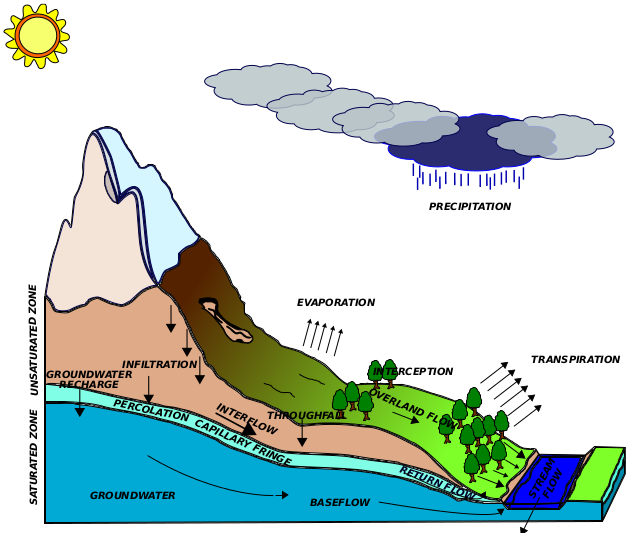
\includegraphics[width=1\textwidth,height=\textheight]{resources/images/geotop_landscape.png}\\
\endcol \begincol{.48\textwidth}
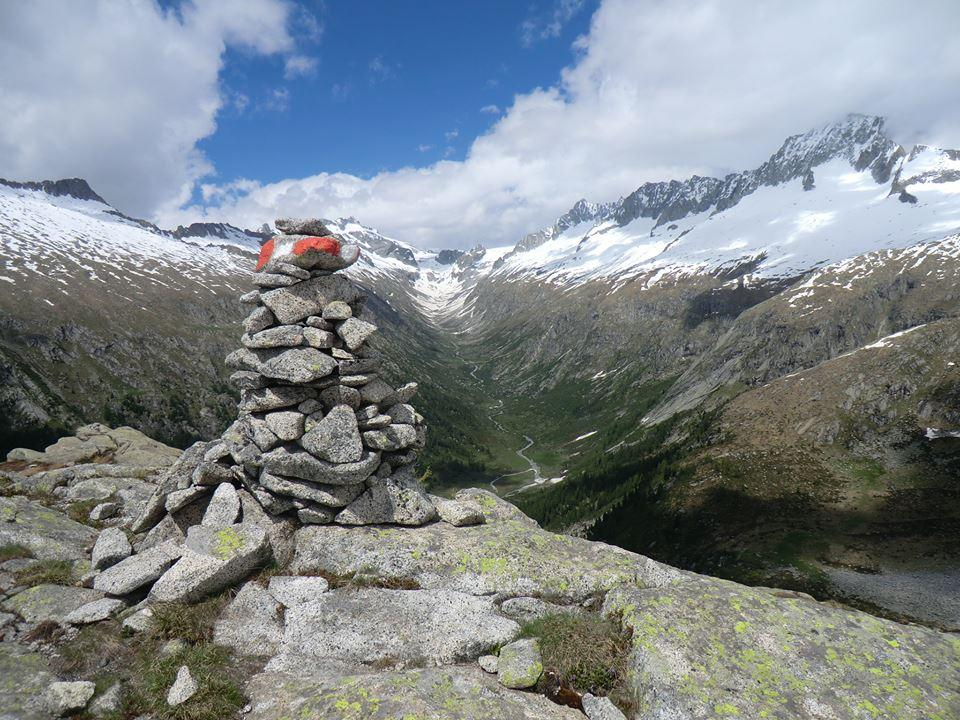
\includegraphics[width=1\textwidth,height=\textheight]{resources/images/valdifumo.jpg}\\
\endcol \endcols
\end{frame}

\begin{frame}{Hydrological Models}
\protect\hypertarget{hydrological-models}{}
\begincols
  \begincol{.58\textwidth}

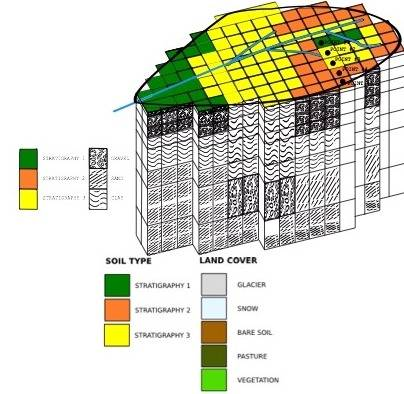
\includegraphics[width=0.7\textwidth,height=\textheight]{resources/images/geotop_grid_mod2.jpg}~
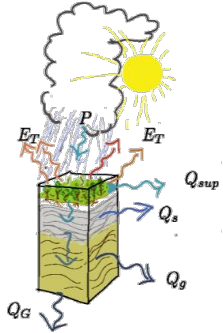
\includegraphics[width=0.5\textwidth,height=\textheight]{resources/images/water_balance.png}\\
\endcol \begincol{.02\textwidth} \endcol \begincol{.36\textwidth}

Models that estimate water river discharge, soil water
content,evapo-transpiration, etc. (\emph{output}) in function of weather
forcings and soil/land/geomorphological characterization (\emph{input}).

\endcol
\endcols

Soil water mass balance equation:
\(\frac{\partial \theta}{\partial t} = \nabla \cdot \left[ K \left(\nabla (\psi+z_f) \right) \right] +S\)

Soil Heat (energy) balance equation:
\(C_s \frac{\partial T_s}{\partial t} = \nabla \cdot \left[ K_t ( \nabla T_s ) \right] +\lambda S\)
\end{frame}

\begin{frame}{GEOtop (www.geotop.org)}
\protect\hypertarget{geotop-www.geotop.org}{}
GEOtop hydrological model is an open-source C/C++ code solveing water
and energy balance equations coupled with the exchanges between terrain
and lower atmoshere:

\begin{itemize}
\item
  \textbf{1D}: only vertical fluxes \(\,\to\,\) balances at local scale
  (only in one soil column)
\item
  \textbf{3D}: vertical and lateral fluxes \(\,\to\,\) balances at basin
  scale
\end{itemize}

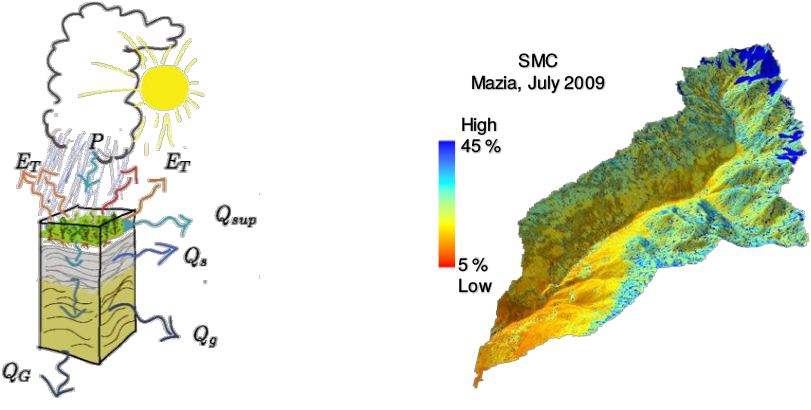
\includegraphics[width=0.6\textwidth,height=\textheight]{resources/images/geotop_ET_SWC.png}\\
\end{frame}

\begin{frame}[fragile]{How can we use GEOtop physical variables in R?
``geotopbricks'' R Package.}
\protect\hypertarget{how-can-we-use-geotop-physical-variables-in-r-geotopbricks-r-package.}{}
\textbf{GEOtop} configuration file, called \textbf{geotop.inpts}
contains keywords addressing to simulation options (e.g.~simulation
period) or pointing to \textbf{input files} (e.g.~meteorological
forcings, soil and geomorphology of the basin) or \textbf{output files}
(spatio-temporal maps - raster and time series - of the results).
\begincols \begincol{.35\textwidth}
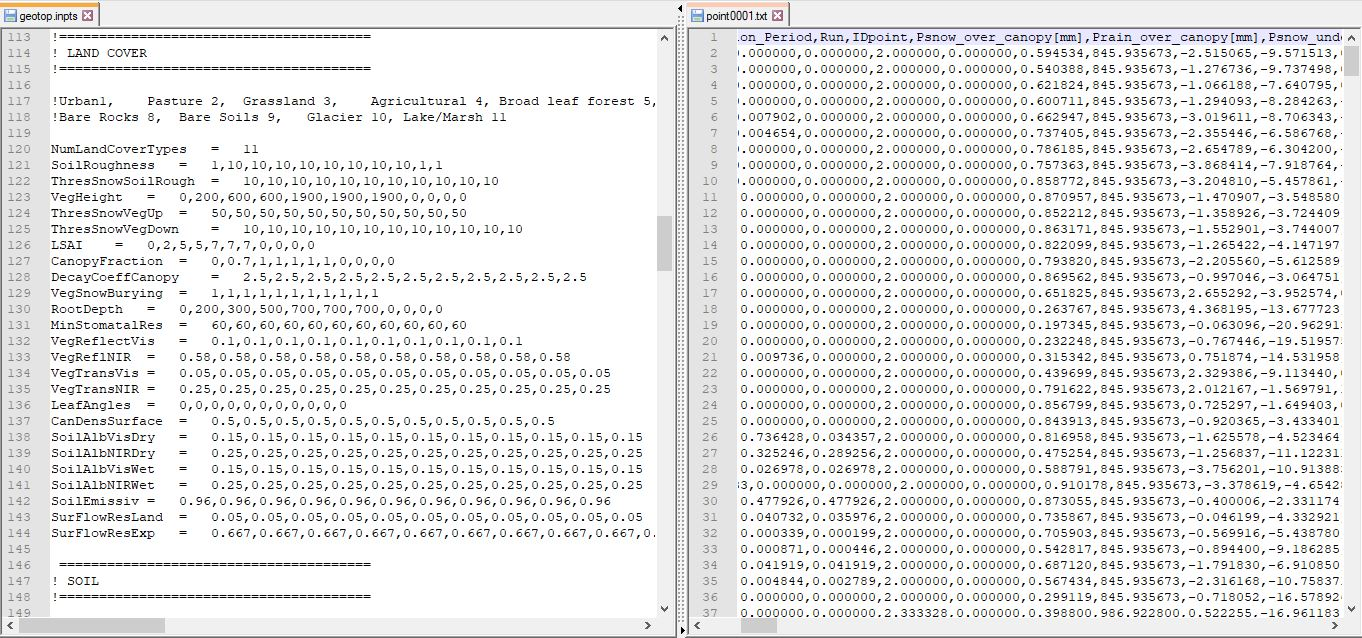
\includegraphics[width=0.9\textwidth,height=\textheight]{resources/images/Capture_IO_GEOtopJPG.JPG}\\

\endcol
\begincol{.65\textwidth}

\begin{verbatim}
InitDateDDMMYYYYhhmm=09/04/2014 18:00  
EndDateDDMMYYYYhhmm =01/01/2016 00:00 
[...] 
MeteoFile           ="meteoB2_irr" 
PointOutputFile     ="tabs/point" 
\end{verbatim}

\endcol
\endcols

\textbf{geotopbricks} parses \textbf{geotop.inpts} and imports
\textbf{GEOtop} data directly into the \emph{R} session.
\end{frame}

\begin{frame}{1D GEOtop Simulation in an Alpine Site: 2 Points}
\protect\hypertarget{d-geotop-simulation-in-an-alpine-site-2-points}{}
Estimation of soil water content (SWC) in two points \textbf{P2} and
\textbf{B2} located in Val Mazia/Matsch, South Tyrol, Italy
\url{http://lter.eurac.edu/en}. \begincols

\begincol{0.30\textwidth}

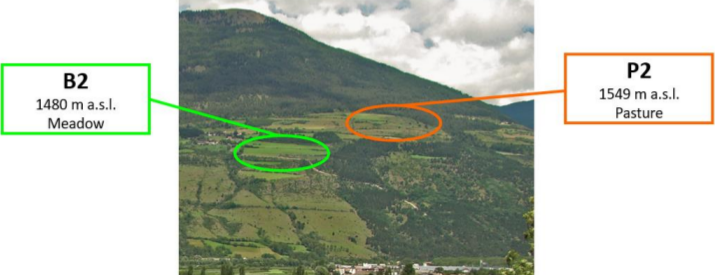
\includegraphics[width=1\textwidth,height=\textheight]{resources/images/B2_P2.png}\\
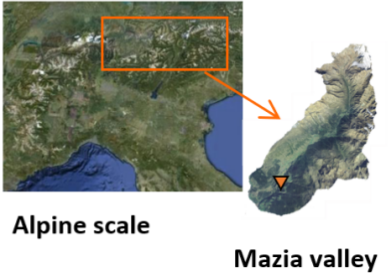
\includegraphics[width=1\textwidth,height=\textheight]{resources/images/mazia_2.png}\\
\endcol \begincol{0.30\textwidth}
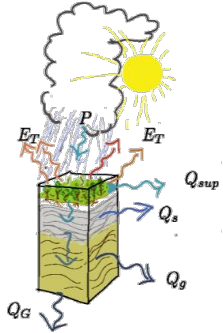
\includegraphics[width=1\textwidth,height=\textheight]{resources/images/water_balance}\\
\endcol \begincol{0.40\textwidth}

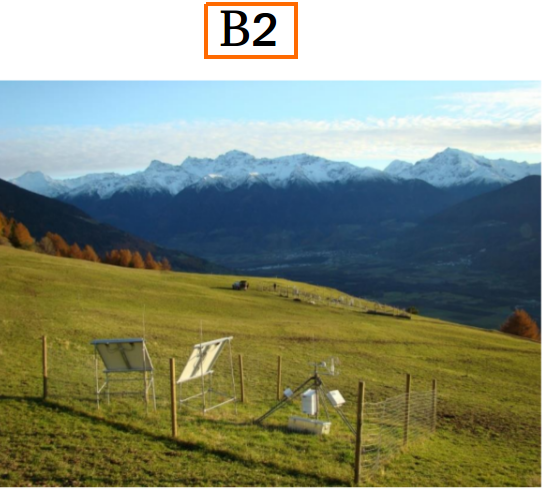
\includegraphics[width=1\textwidth,height=\textheight]{resources/images/B2_new.png}\\
\endcol \endcols
\end{frame}

\begin{frame}[fragile]{1D GEOtop Simulation in an Alpine Site: B2}
\protect\hypertarget{d-geotop-simulation-in-an-alpine-site-b2}{}
Here is the directory containing files of B2 point simulation:

\begin{Shaded}
\begin{Highlighting}[]
\KeywordTok{library}\NormalTok{(geotopbricks) }

\CommentTok{\#\# SET GEOTOP SIMULATION DIRECTORY}
\NormalTok{wpath\_B2 <{-}}\StringTok{ "resources/simulation/Matsch\_B2\_Ref\_007"} 
\end{Highlighting}
\end{Shaded}

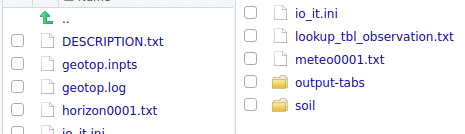
\includegraphics[width=1\textwidth,height=\textheight]{resources/images/geotop_folder_B2.png}\\
\end{frame}

\begin{frame}[fragile]{Getting Simulation Input Data}
\protect\hypertarget{getting-simulation-input-data}{}
Meteorological forcings time series are imported and saved as
\textbf{meteo} variable (class \textbf{zoo}). This variable is retrieved
through the GEOtop keyword \textbf{MeteoFile} :

\begin{Shaded}
\begin{Highlighting}[]
\NormalTok{tz <{-}}\StringTok{ "Etc/GMT{-}1"}
\NormalTok{meteo <{-}}\StringTok{ }\KeywordTok{get.geotop.inpts.keyword.value}\NormalTok{(}
  \StringTok{"MeteoFile"}\NormalTok{,}
  \DataTypeTok{wpath=}\NormalTok{wpath\_B2,}
  \DataTypeTok{data.frame=}\OtherTok{TRUE}\NormalTok{,}
  \DataTypeTok{tz=}\NormalTok{tz)}
\KeywordTok{class}\NormalTok{(meteo)}
\end{Highlighting}
\end{Shaded}

\begin{verbatim}
## [1] "zoo"
\end{verbatim}
\end{frame}

\begin{frame}{Precipitation and Air Temperature at B2}
\protect\hypertarget{precipitation-and-air-temperature-at-b2}{}
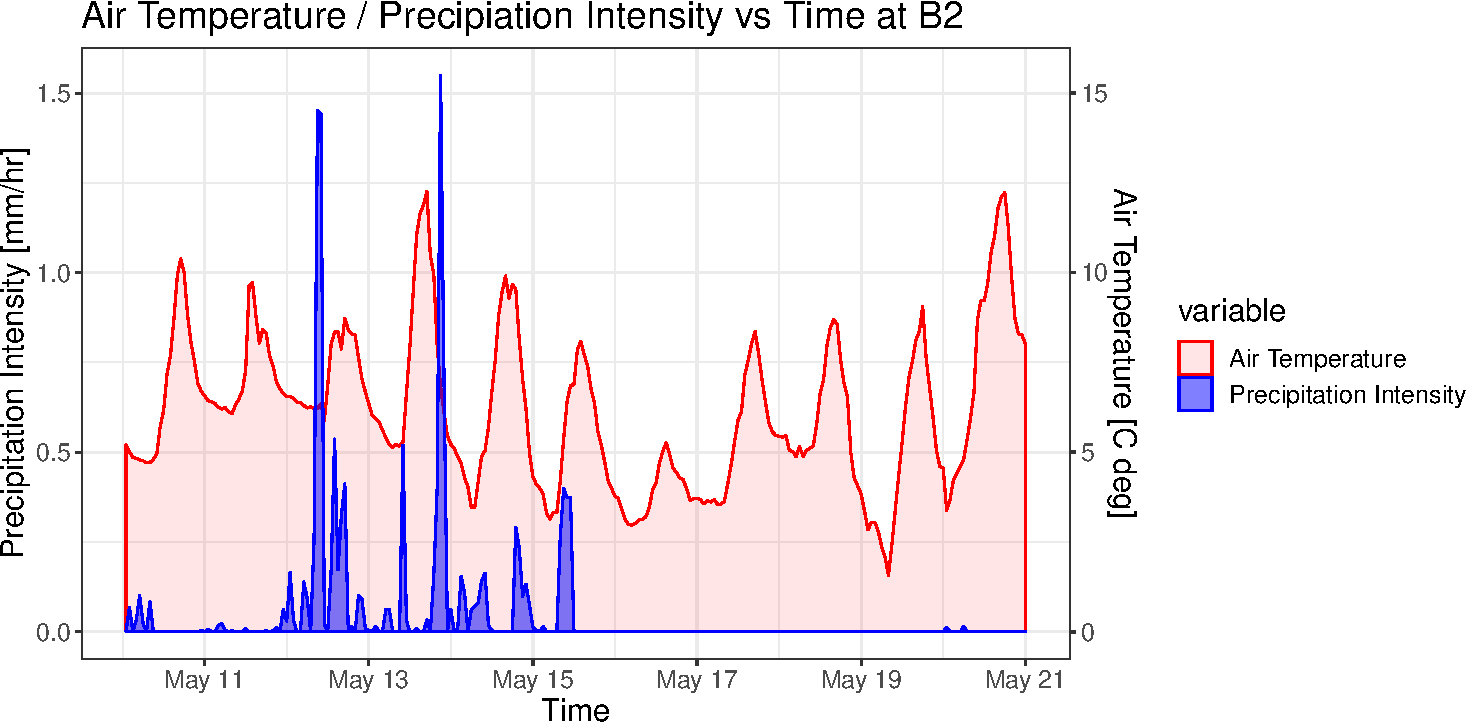
\includegraphics{presentation_files/figure-beamer/unnamed-chunk-3-1.pdf}
\end{frame}

\begin{frame}[fragile]{Getting Simulation Output Data}
\protect\hypertarget{getting-simulation-output-data}{}
Soil Water Content Profile:

\begin{Shaded}
\begin{Highlighting}[]
\NormalTok{tz <{-}}\StringTok{ "Etc/GMT{-}1"}
\NormalTok{SWC\_B2  <{-}}\StringTok{ }\KeywordTok{get.geotop.inpts.keyword.value}\NormalTok{(}
  \StringTok{"SoilLiqContentProfileFile"}\NormalTok{,}
  \DataTypeTok{wpath =}\NormalTok{ wpath\_B2,}
  \DataTypeTok{data.frame =} \OtherTok{TRUE}\NormalTok{,}
  \DataTypeTok{date\_field =} \StringTok{"Date12.DDMMYYYYhhmm."}\NormalTok{,}
  \DataTypeTok{tz =}\NormalTok{ tz,}
  \DataTypeTok{zlayer.formatter =} \StringTok{"z\%04d"}
\NormalTok{)}
\KeywordTok{help}\NormalTok{(get.geotop.inpts.keyword.value) }\CommentTok{\#\# for more details!}
\end{Highlighting}
\end{Shaded}
\end{frame}

\begin{frame}[fragile]{Getting Simulation Output Data (at P2)}
\protect\hypertarget{getting-simulation-output-data-at-p2}{}
Analogously for P2:

\begin{Shaded}
\begin{Highlighting}[]
\NormalTok{wpath\_P2 <{-}}\StringTok{ "resources/simulation/Matsch\_P2\_Ref\_007"} 
\NormalTok{SWC\_P2  <{-}}\StringTok{ }\KeywordTok{get.geotop.inpts.keyword.value}\NormalTok{(}
  \StringTok{"SoilLiqContentProfileFile"}\NormalTok{,}
  \DataTypeTok{wpath =}\NormalTok{ wpath\_P2,}
  \DataTypeTok{data.frame =} \OtherTok{TRUE}\NormalTok{,}
  \DataTypeTok{date\_field =} \StringTok{"Date12.DDMMYYYYhhmm."}\NormalTok{,}
  \DataTypeTok{tz =} \StringTok{"Etc/GMT{-}1"}\NormalTok{,}
  \DataTypeTok{zlayer.formatter =} \StringTok{"z\%04d"}\NormalTok{)}
\end{Highlighting}
\end{Shaded}
\end{frame}

\begin{frame}{Soil Water Content at P2 and B2}
\protect\hypertarget{soil-water-content-at-p2-and-b2}{}
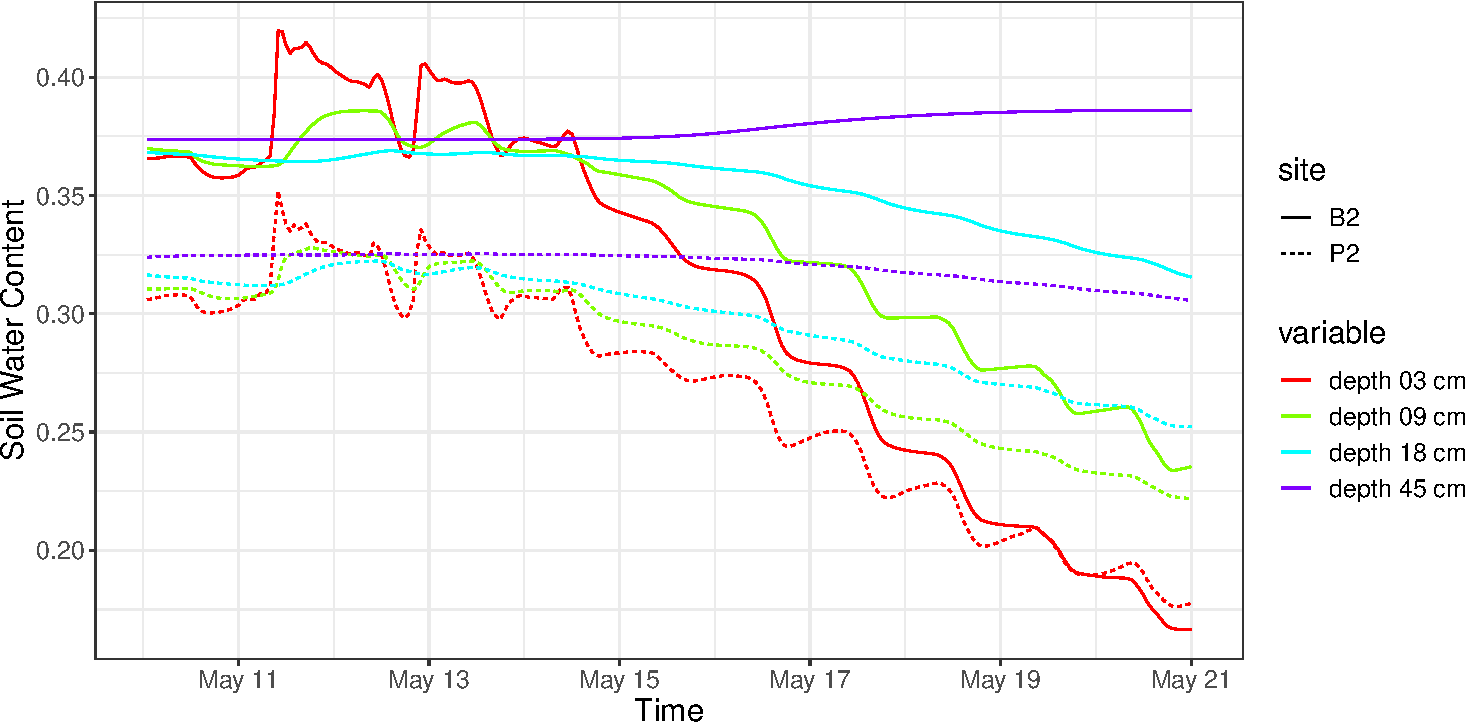
\includegraphics{presentation_files/figure-beamer/unnamed-chunk-8-1.pdf}
\end{frame}

\begin{frame}[fragile]{3D Spatially Distributed Simulation: Val
Venosta/Vinschgau - Upper Adige River Basin - Alps - I/CH/A}
\protect\hypertarget{d-spatially-distributed-simulation-val-venostavinschgau---upper-adige-river-basin---alps---icha}{}
\begin{Shaded}
\begin{Highlighting}[]
\NormalTok{wpath\_3D <{-}}\StringTok{ \textquotesingle{}resources/simulation/Vinschgau\textquotesingle{}}
\NormalTok{basin <{-}}\StringTok{ }\KeywordTok{get.geotop.inpts.keyword.value}\NormalTok{(}\StringTok{"LandCoverMapFile"}\NormalTok{,}
              \DataTypeTok{wpath=}\NormalTok{wpath\_3D,}\DataTypeTok{raster=}\OtherTok{TRUE}\NormalTok{)}
\NormalTok{basin}
\end{Highlighting}
\end{Shaded}

\begin{verbatim}
## class      : RasterLayer 
## dimensions : 48, 63, 3024  (nrow, ncol, ncell)
## resolution : 1000, 1000  (x, y)
## extent     : 598000, 661000, 5145000, 5193000  (xmin, xmax, ymin, ymax)
## crs        : +proj=utm +zone=32 +ellps=WGS84 +datum=WGS84 +units=m +no_defs +towgs84=0,0,0 
## source     : memory
## names      : layer 
## values     : 1, 11  (min, max)
\end{verbatim}
\end{frame}

\begin{frame}{Input GeoSpatial Map: Elevation and Weather Station}
\protect\hypertarget{input-geospatial-map-elevation-and-weather-station}{}
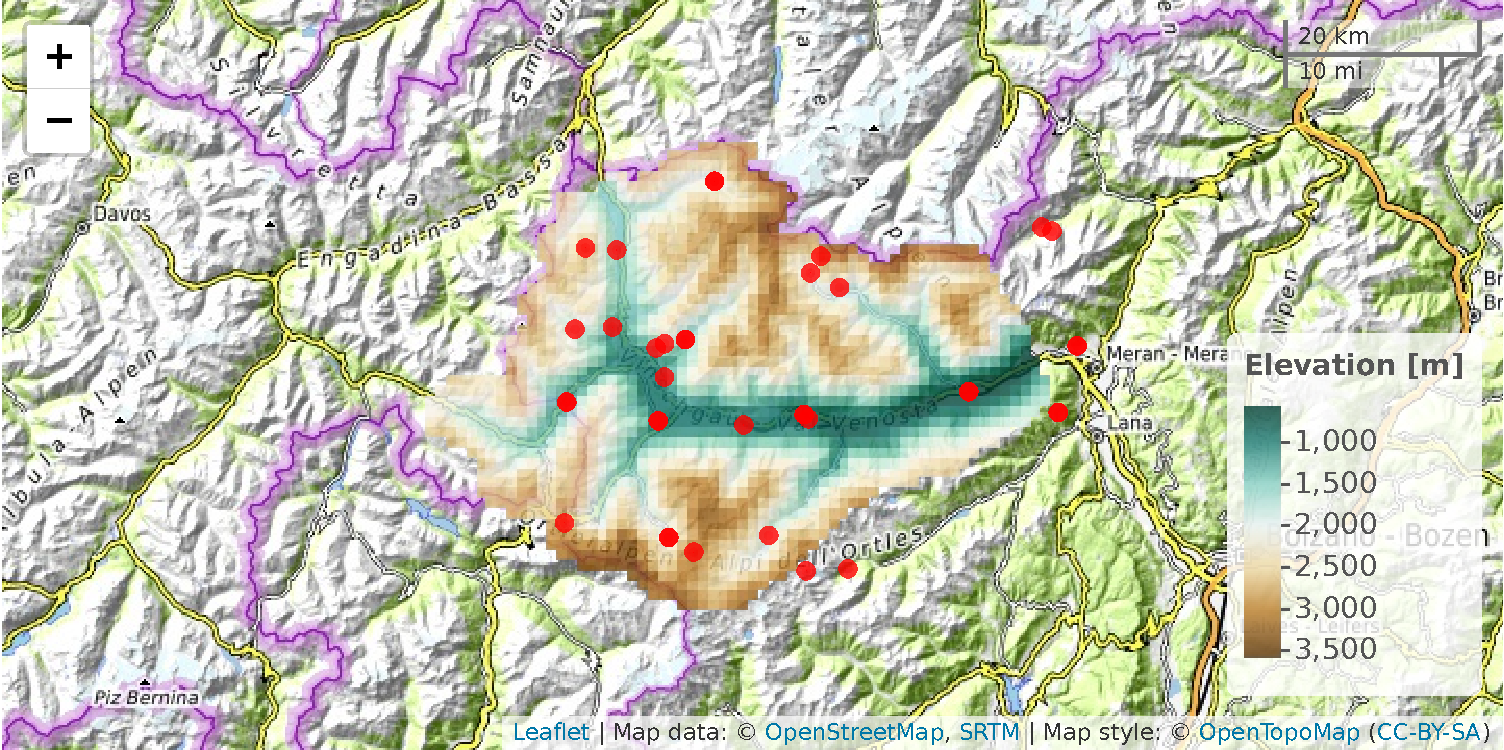
\includegraphics{presentation_files/figure-beamer/unnamed-chunk-10-1.pdf}
\end{frame}

\begin{frame}[fragile]{3D Spatially Distributed Simulation (Output
Geospatial Map): Soil Water Content}
\protect\hypertarget{d-spatially-distributed-simulation-output-geospatial-map-soil-water-content}{}
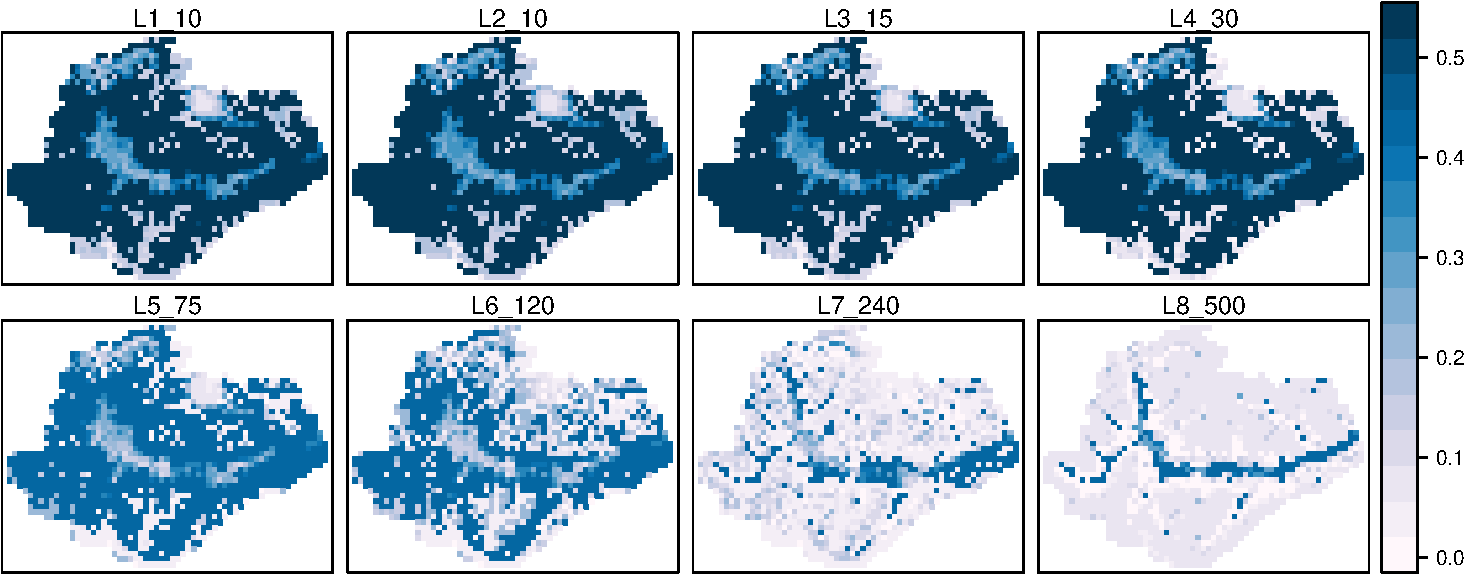
\includegraphics{presentation_files/figure-beamer/unnamed-chunk-11-1.pdf}

\begin{verbatim}
brickFromOutputSoil3DTensor("SoilLiqContentTensorFile", 
wpath=wpath_3D,when="2011-08-16 12:00:00 +01")
\end{verbatim}
\end{frame}

\begin{frame}{3D Spatially Distributed Simulation (Output Geospatial
Map): Surface Water Discharge at the Outlet}
\protect\hypertarget{d-spatially-distributed-simulation-output-geospatial-map-surface-water-discharge-at-the-outlet}{}
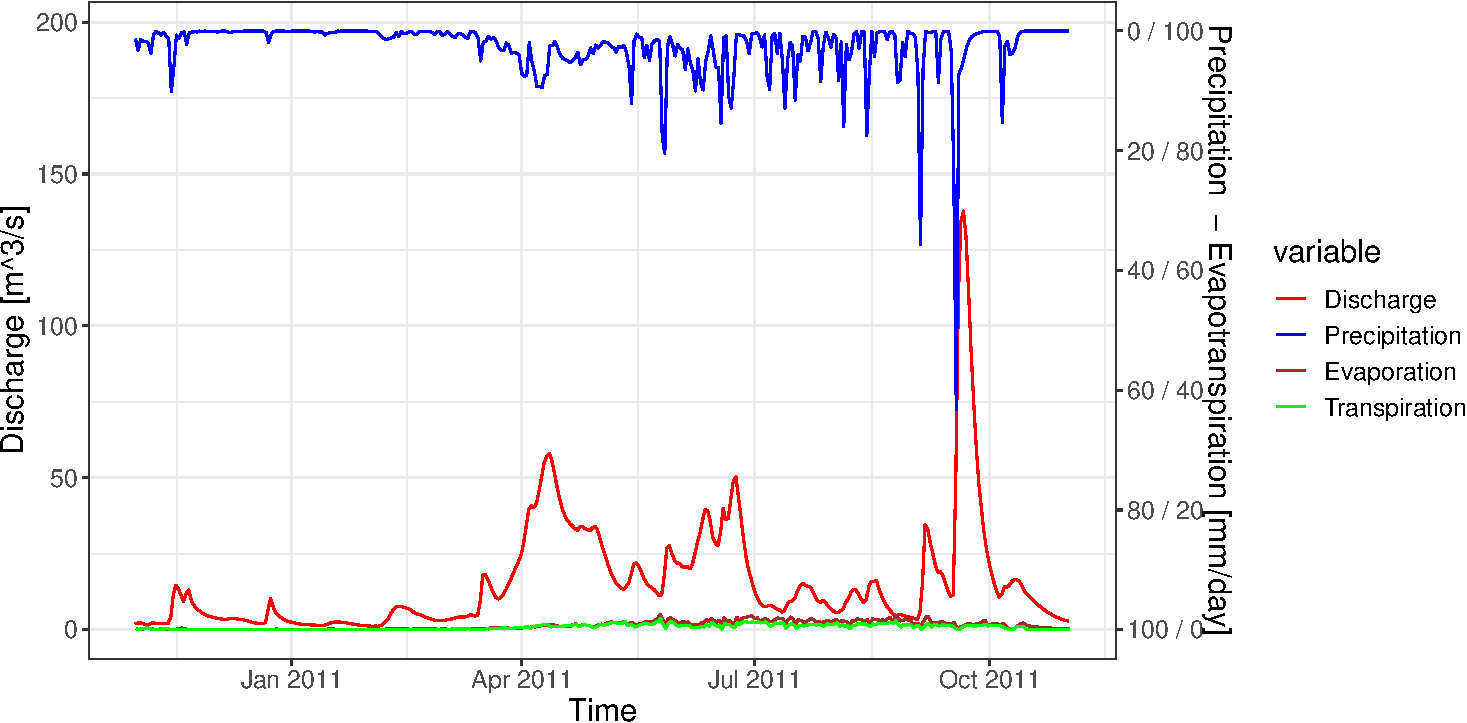
\includegraphics{presentation_files/figure-beamer/unnamed-chunk-13-1.pdf}
\end{frame}

\begin{frame}{Application: snow cover modelling}
\protect\hypertarget{application-snow-cover-modelling}{}
Occurrence of large herbivore depending on feeding station location and
\textbf{snow cover}:

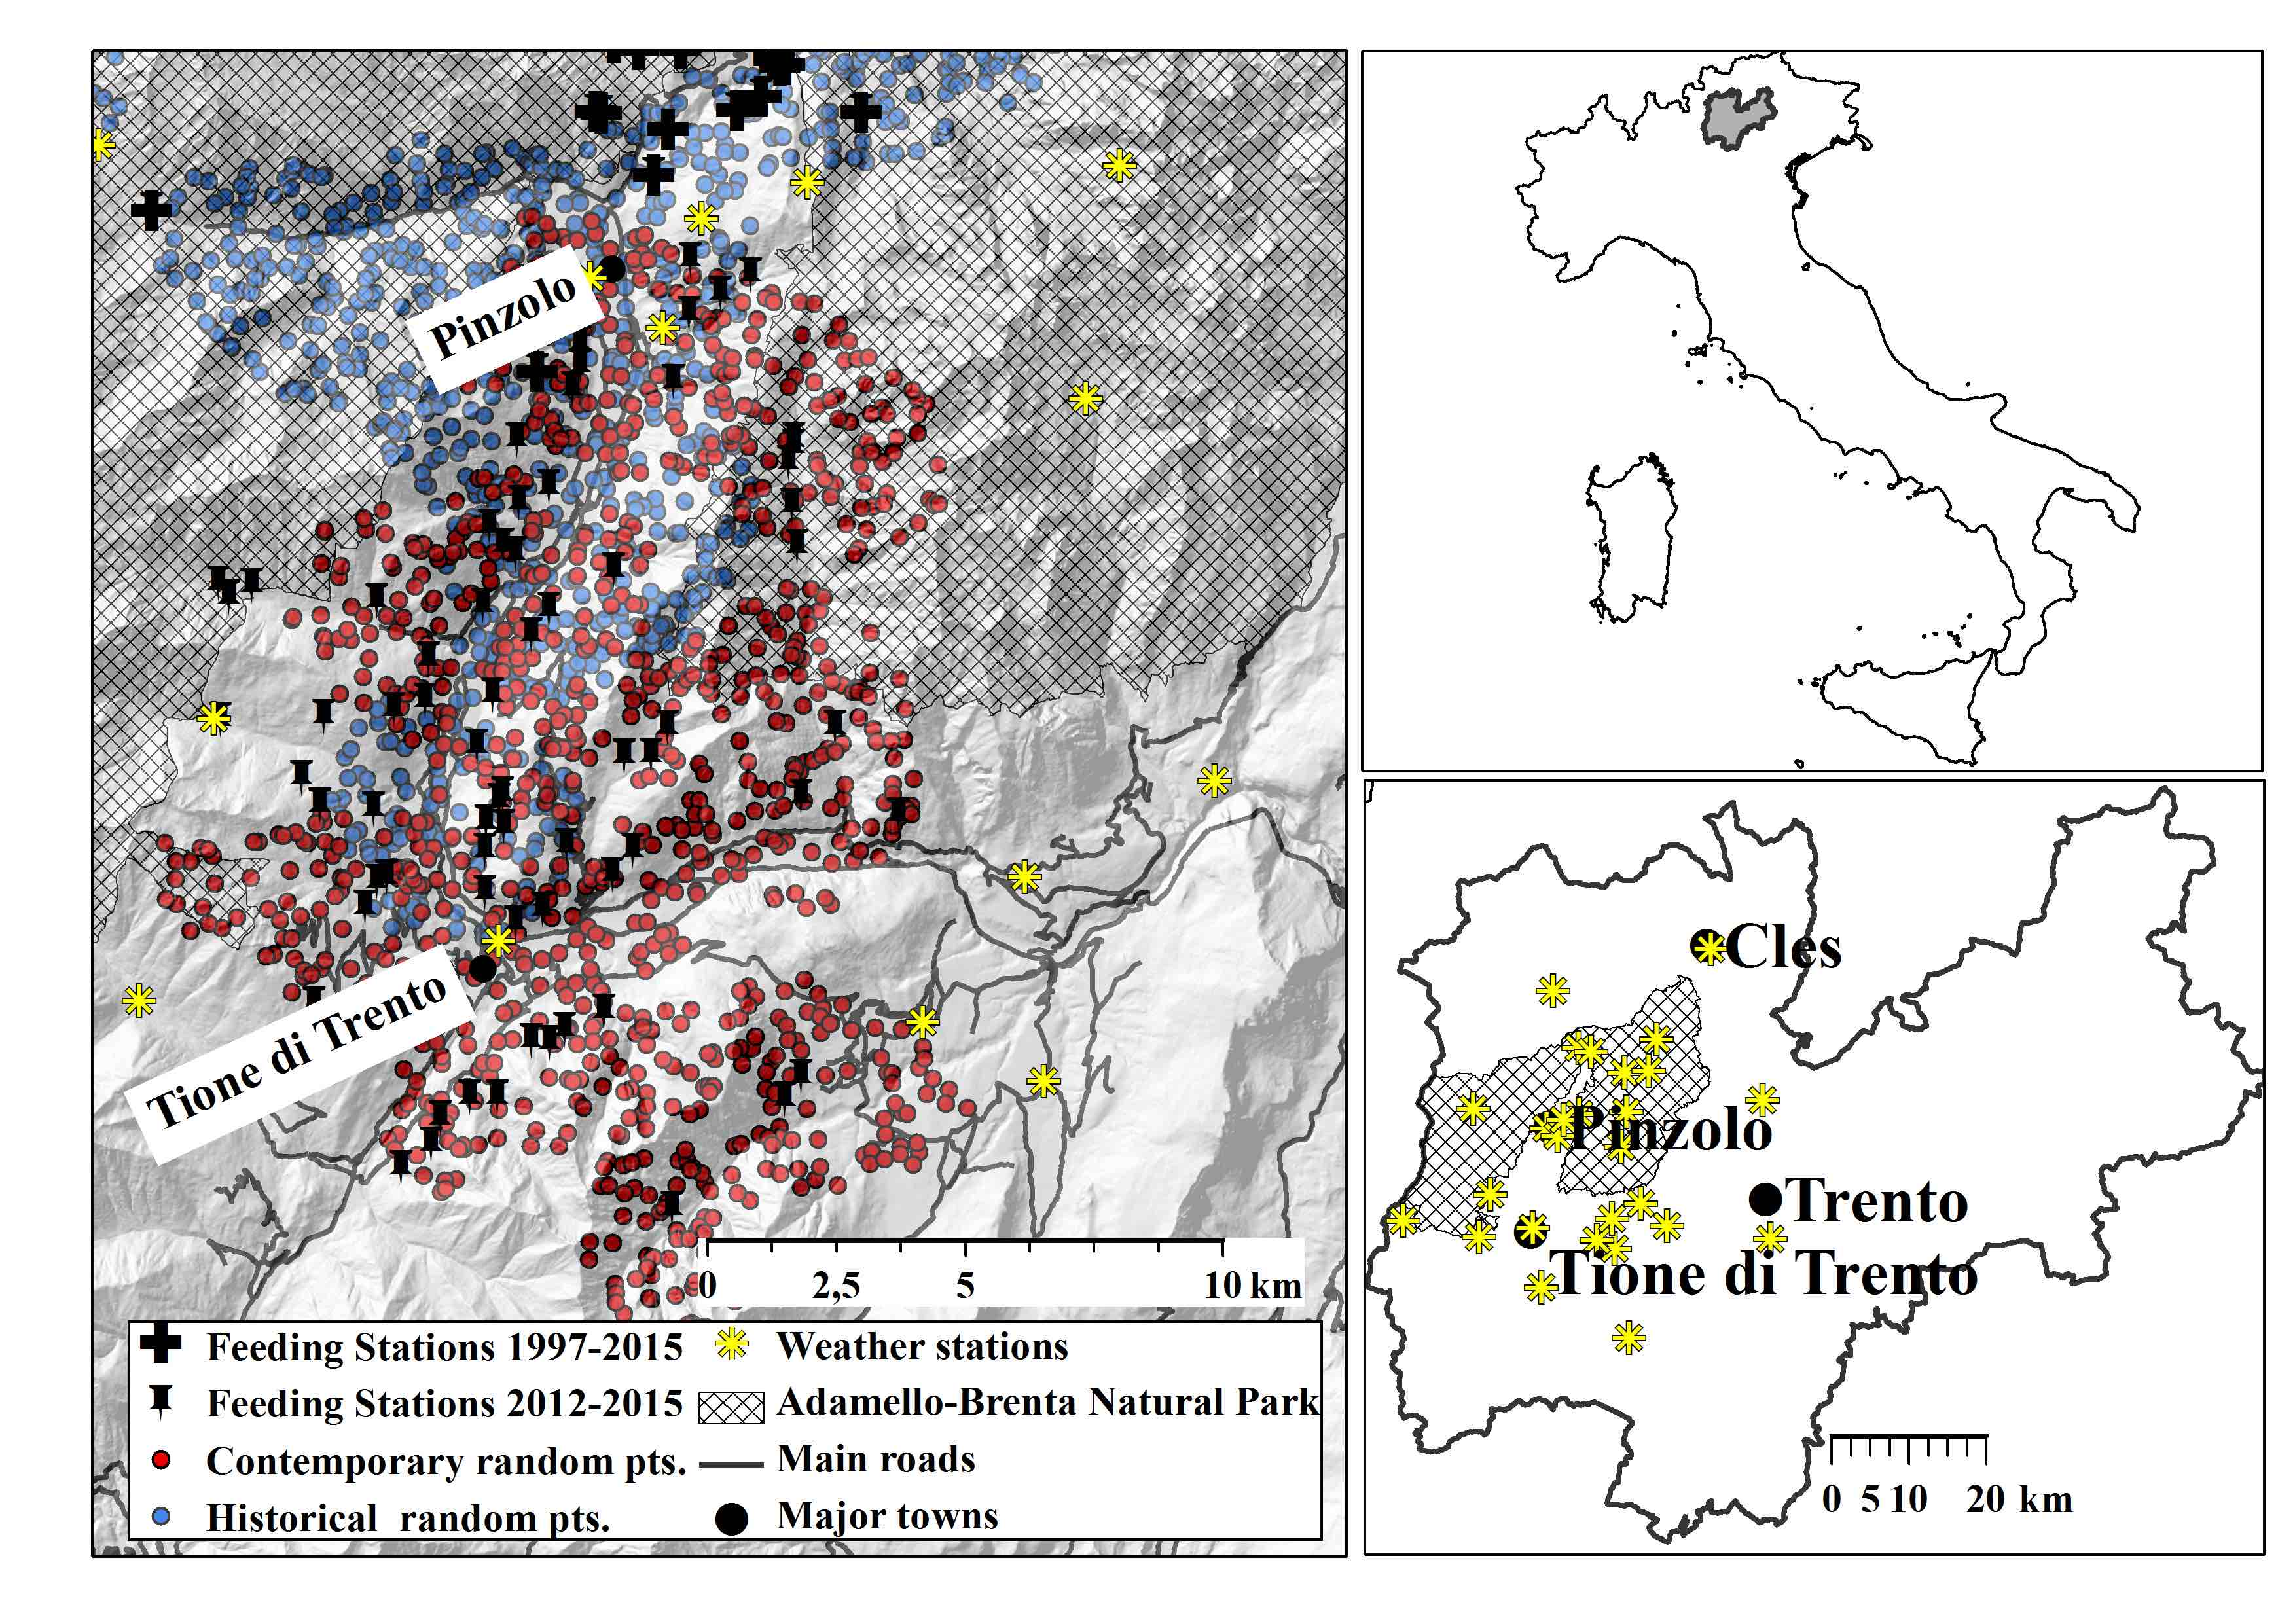
\includegraphics[width=0.7\textwidth,height=\textheight]{resources/images/rendena_roe_deer_meteo_v2.jpg}\\
\end{frame}

\begin{frame}{Snow Spatial Distribution in Winter (DJFM)}
\protect\hypertarget{snow-spatial-distribution-in-winter-djfm}{}
\begin{longtable}[]{@{}lll@{}}
\toprule
Winter & Mean Depth {[}mm{]} & Duration {[}days{]}\tabularnewline
\midrule
\endhead
2013-2014 &
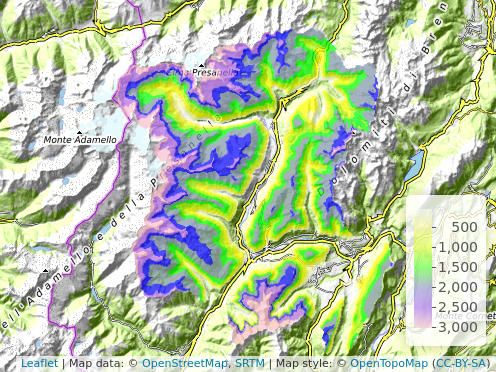
\includegraphics[width=\textwidth,height=1.04167in]{resources/images/map/mean_OBS_2014_winter.png}
&
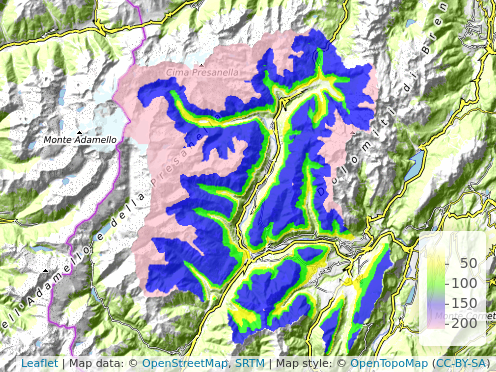
\includegraphics[width=\textwidth,height=1.04167in]{resources/images/map/nday_OBS_2014_winter.png}\tabularnewline
2014-2015 &
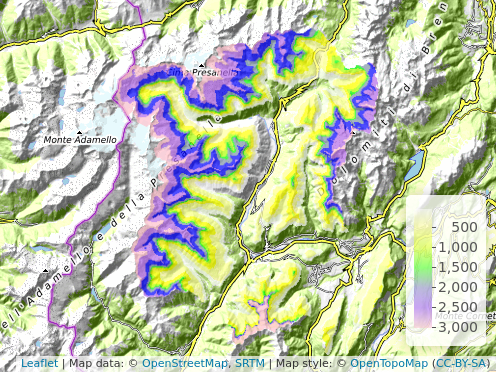
\includegraphics[width=\textwidth,height=1.04167in]{resources/images/map/mean_OBS_2015_winter.png}
&
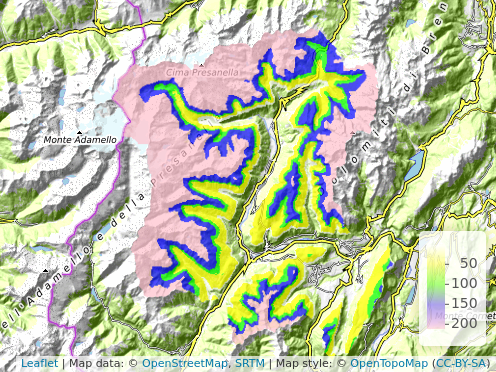
\includegraphics[width=\textwidth,height=1.04167in]{resources/images/map/nday_OBS_2015_winter.png}\tabularnewline
\bottomrule
\end{longtable}
\end{frame}

\begin{frame}{Snow Depth and Cover Variabilty}
\protect\hypertarget{snow-depth-and-cover-variabilty}{}
Summarize snow depth and snow cover during a winter season versus
elevation:

\begin{center}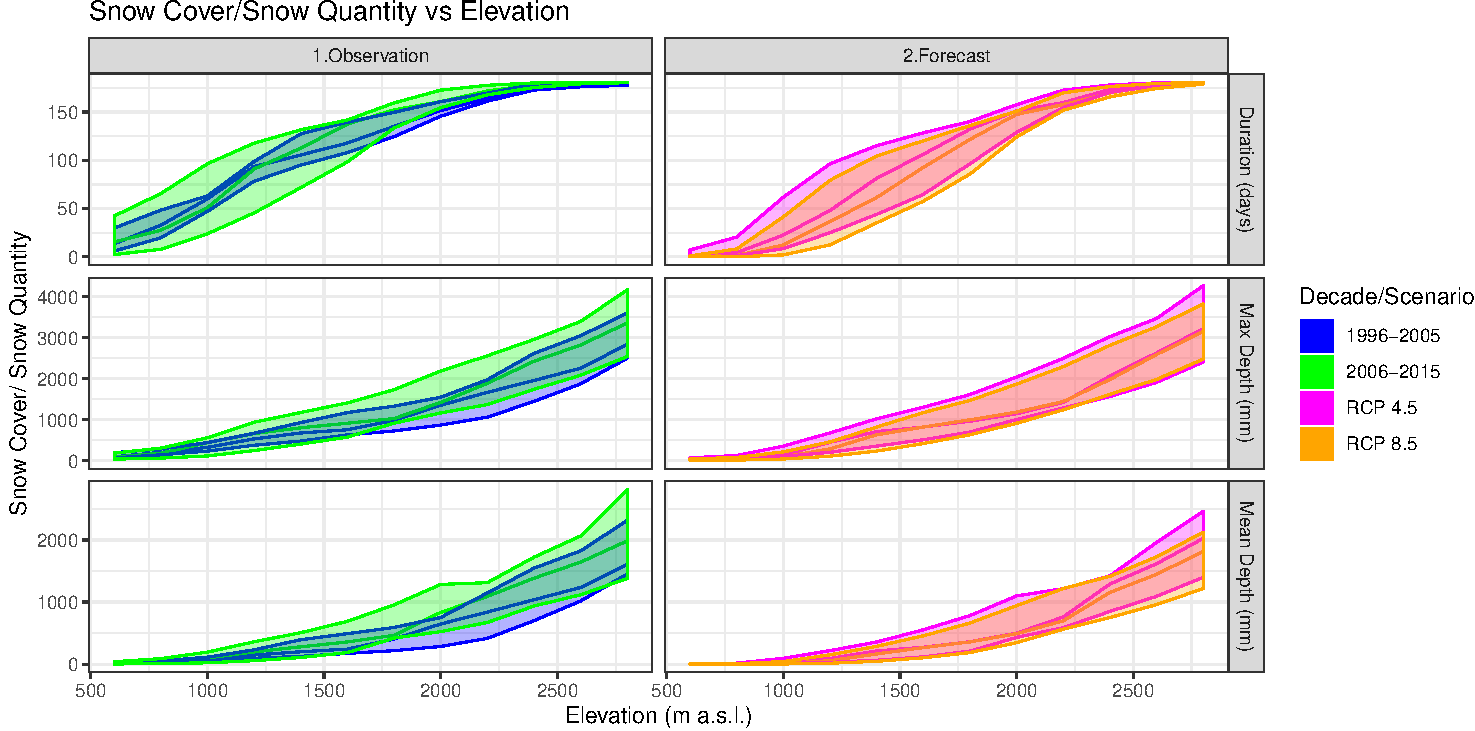
\includegraphics[width=0.9\linewidth]{presentation_files/figure-beamer/snow-altitude-1} \end{center}
\end{frame}

\begin{frame}{Final Remarks}
\protect\hypertarget{final-remarks}{}
\begin{itemize}
\item
  \textbf{geotopbricks} is an interface of GEOtop in R speaking the
  language of GEOtop;
\item
  Through \textbf{geotopbricks} user can interact between R and GEOtop
  using R enviroment and GEOtop keywords system, without getting crazy
  to search files thoughout the specific GEOtop simulation structure;
\end{itemize}

\begin{itemize}
\tightlist
\item
  This presentation has been created as a \textbf{RMarkdown} living and
  reproducible document, all shown results from GEOtop model have been
  automatically imported and plotted.
\end{itemize}
\end{frame}

\begin{frame}{Acknowledgments to GEOtop and R contributors, Thank you
for your attention and some tips about us\ldots{}}
\protect\hypertarget{acknowledgments-to-geotop-and-r-contributors-thank-you-for-your-attention-and-some-tips-about-us}{}
\begincols

\begincol{0.28\textwidth}

Me
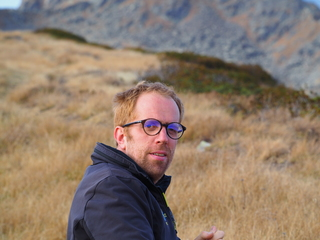
\includegraphics[width=1\textwidth,height=\textheight]{resources/images/emanuele.jpg}~

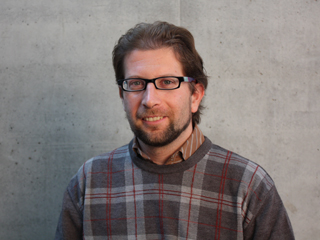
\includegraphics[width=0.7\textwidth,height=\textheight]{resources/images/giacomo.jpg}\\
Dr.~Giacomo Bertoldi \endcol

\begincol{0.7\textwidth}

\begin{itemize}
\item
  I'm an Environmental engineer with hydrological background (more
  deterministic and physically-based than statics!) freelancer, -
  www.rendena100.eu . I'm author of several R-packages and R enthusiast.
\item
  I work in collaboration with adevanced users and developer of GEOtop
  hydrologic models with skills in hydrology, environmental science and
  also in C/C++, parallell programming, High Perfomance Computing, etc.
\end{itemize}

\endcol

\endcols
\end{frame}

\begin{frame}{Addendum}
\protect\hypertarget{addendum}{}
\end{frame}

\begin{frame}{GEOtop Hydrological Model Flowchart}
\protect\hypertarget{geotop-hydrological-model-flowchart}{}
\begincols

\begincol{.69\textwidth}

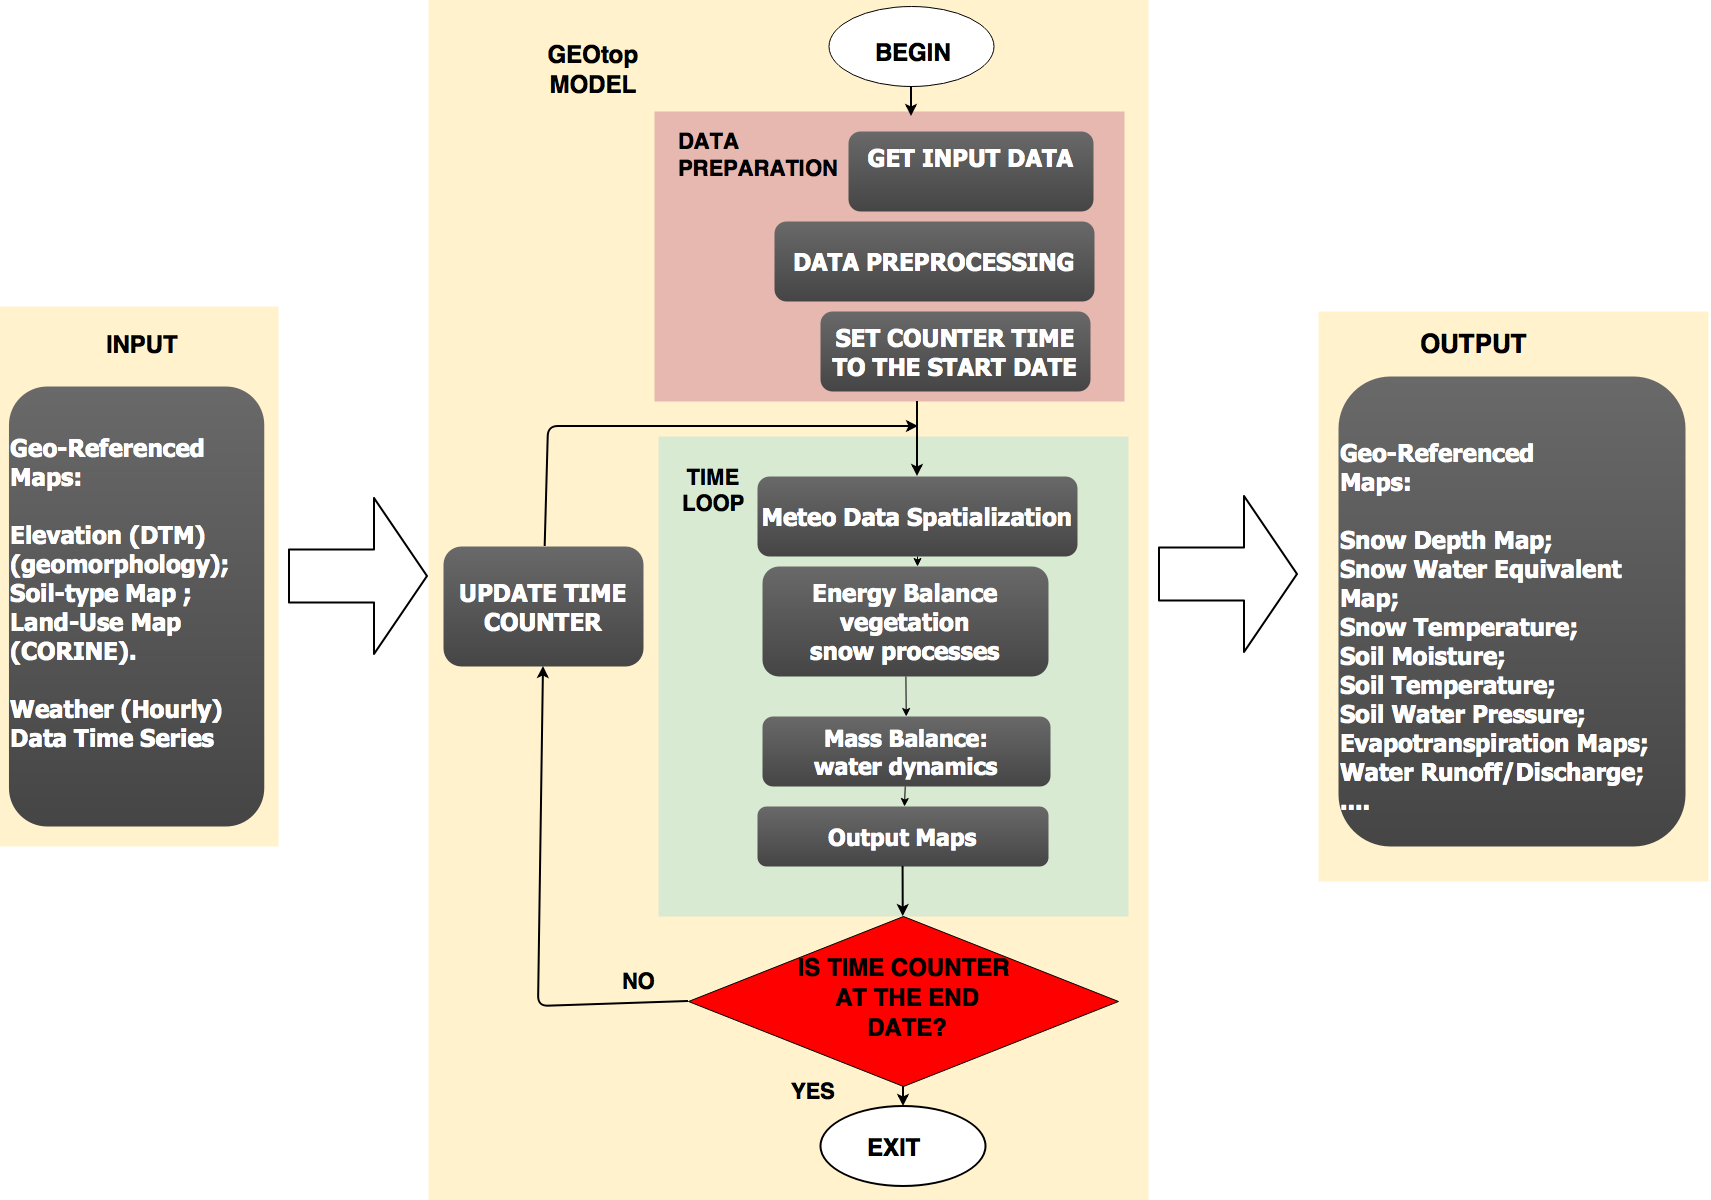
\includegraphics[width=1\textwidth,height=\textheight]{resources/images/geotop_revised.png}\\
\endcol

\begincol{.30\textwidth}

\begin{itemize}
\item
  \textbf{Input}: meteo data, elevations, soil parameters,\ldots{}
\item
  \textbf{Output}: snow cover, soil temperature, soil moisture,\ldots{}
\end{itemize}

\endcol
\endcols
\end{frame}

\begin{frame}{Soil Water Pressure Head at P2 and B2}
\protect\hypertarget{soil-water-pressure-head-at-p2-and-b2}{}
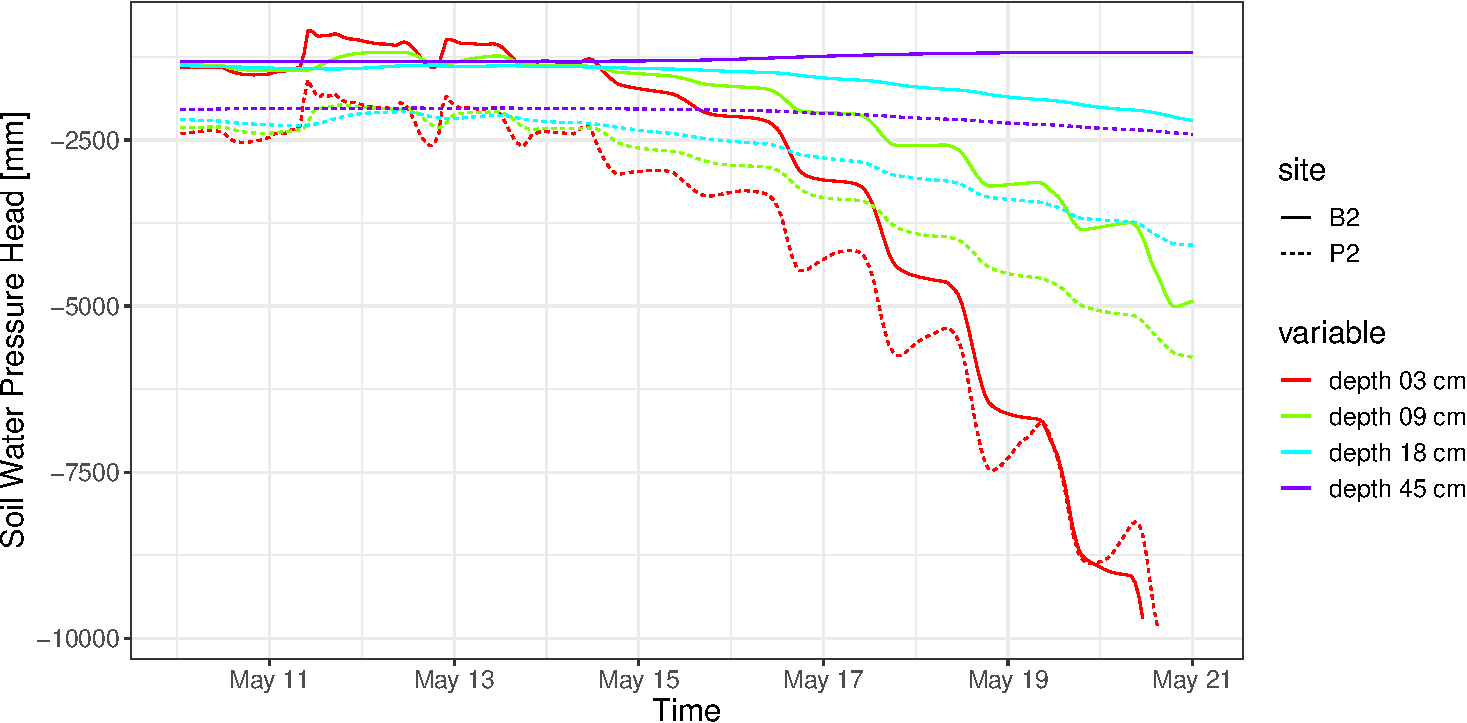
\includegraphics{presentation_files/figure-beamer/unnamed-chunk-14-1.pdf}
\end{frame}

\begin{frame}{Example of an Output Data Analytics (Soil Moisture
Distribution)}
\protect\hypertarget{example-of-an-output-data-analytics-soil-moisture-distribution}{}
Distribution of daily aggregated soil water contant at a 18 cm depth:
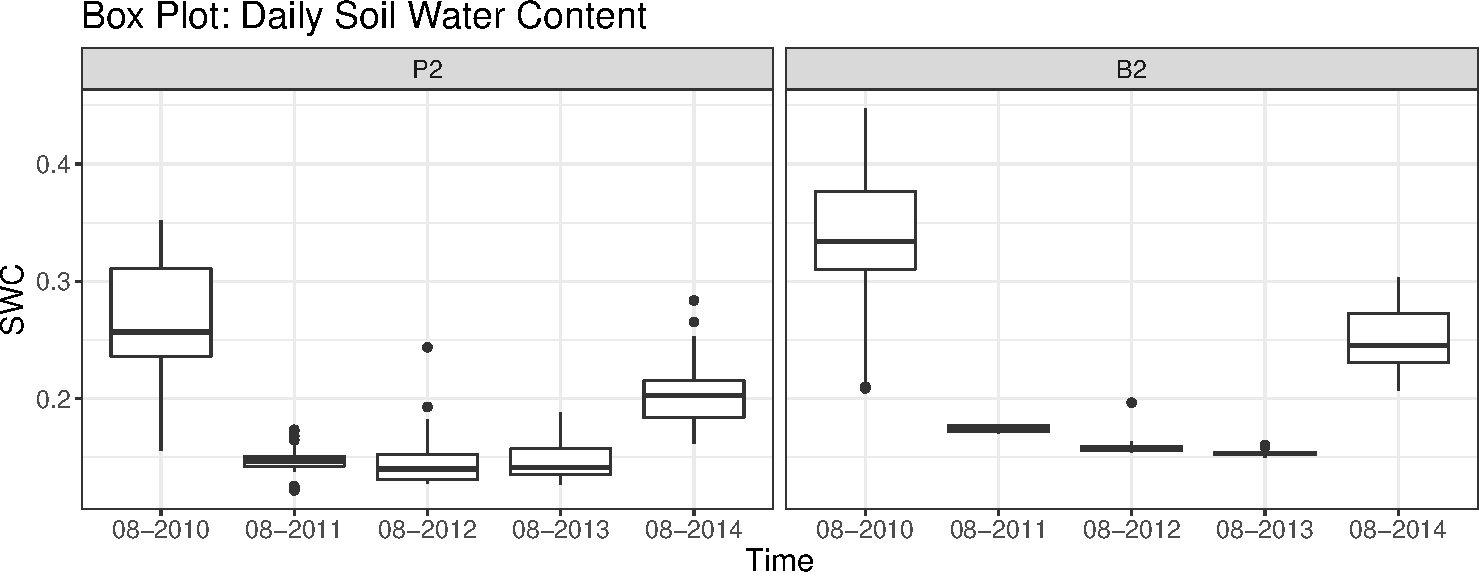
\includegraphics{presentation_files/figure-beamer/unnamed-chunk-15-1.pdf}
\end{frame}

\end{document}
